\section{Method}
\label{ch:method}
This chapter presents our method for constructing efficient multi-mode architectures. We start by considering possible efficiency metrics and their applicability in our case to answer RQ1. Next, we present the actual merging method, which combines two application-specific architectures, thus answering RQ2. Finally, we extend this method with a DSE, to find pairings within the sets of input architectures that result in efficient merged architectures, answering RQ3.

\section{Efficiency metrics}
The first step in our research is to establish which metrics to consider for efficiency. Doing so helps guide the creation of our method towards a shared goal, helping us decide the input and steps our method should take in order to best optimise these metrics.

We base our discussion on latency, area usage, and energy consumption, as these metrics are the most common in the HLS and DSE literature seen so far. The latency of an architecture represents the time needed to execute the program it implements, measured in clock cycles. Area usage refers to the amount of physical area required to implement the architecture on a chip. Lastly, the energy consumption is the amount of energy required to execute the application, and is divided into the passive energy, determined by passive leakage of electrical energy in hardware, and the dynamic energy, required to activate the components.

Out of these, area is the most important metric to us, as we are specifically aiming to design a merging method that exploits resource sharing. Because area is determined by component count and size, and the goal of resource sharing is to avoid unnecessary resource duplication, minimising the area of the merged architecture implies maximising resource re-use. Thus, our method aims to optimise the area of the merged architecture.

In contrast, the latency of the input applications in the output architecture is directly related to their latency in the original architectures. By selecting architectures with higher latencies, we can use less parallel and thus lower area architectures in our merge. To explore the different combinations of latency and area, we rely on the latency of the original architecture, and make use of the DSE process to select the pairs of architectures to merge.

Finally, energy is made up of two components, the static and dynamic energy. The dynamic energy of an application is determined mostly by the amount of operations in the application, and is thus largely constant regardless of architecture. On the other hand, the static energy is determined by the passive leakage of the hardware, and only depends on the area and latency. Because a merged architecture is larger than its inputs, running a program on a merged architecture incurs an energy overhead compared to running it on its original architecture. Thus, the energy consumption of the architecture is highly dependent on the values of the latency and area.

In conclusion, when merging input architectures, we prioritise minimising the area of the merged architecture, while preserving the latency of the input architectures, and minimising energy consumption.

\section{Merging method for architectures}
\label{method:method}
Our goal is to devise a method to merge two application-specific architectures as output by the \microgenie framework. The resulting architecture must be able to run each application individually, and minimise area and static energy while preserving the latency and dynamic energy of the original input architectures. We note that it is not necessary for applications to be able to run concurrently, as our goal is to be able to run \textit{either} application on the same hardware, rather than \textit{both} at the same time. We focus on creating the necessary \textit{hardware}, relying on a separate step to create the necessary hardware instructions to run the input applications on the merged hardware.

To meet these requirements, our method that merges two architectures, represented as graphs of FUs, has three major steps:
\begin{enumerate}
\item Isolate the maximum common subgraph \textit{mcs} of the input graphs.
\item Mapping the `leftover' nodes where possible.
\item Completing the graph with the remaining `leftovers'.
\end{enumerate}
We further present the motivation and procedure for each of these steps.

\subsection{Isolating the \textit{mcs}}
We begin the merge by isolating the \textit{mcs} of the input graphs to use as the `core' of our merged architecture. By definition, this is a subgraph that exists within both input graphs that is also maximum in its size compared to other common subgraphs. Thus, the \textit{mcs} represents the largest part of the input architectures that we can directly reuse in our result without introducing any additional hardware or overhead, as it is used in both original architectures. We note that multiple \textit{mcs} of equal size may exist for any pair of architectures, any one of these are valid for our method.

We solve the \textit{mcs} by transforming it to the maximum clique problem on the compatibility graph of the input graphs (as outlined in Section~\ref{bg:mcs}). We impose an additional restriction to the \textit{mcs} found in this manner: two FUs can only map onto each other if they perform the same operation in hardware. Because we rely on a separate step to implement the input applications on the merged hardware, we do not consider the instruction memory in the FUs for this restriction.

\subsection{Mapping leftovers}
After isolating the \textit{mcs}, we are left with two sets of `leftover' nodes. Our next step is to map together---that is, map on shared resources---any nodes of the same type between the two leftover sets. Pairing two nodes from the two different sets, and mapping each pair on a new shared resource creates \textit{one} new node in our merged graph, with all of the connections of both original nodes.

Matching these leftovers results in new nodes with edges that should only be active when one of the two applications is running, meaning that we must be able to ignore certain hardware connections at runtime. This is possible by adding switching hardware where these edges meet, allowing the hardware to select which of multiple inputs to connect to an output. In the FUs used in our framework, this functionality is provided by the crossbar.

Compared to the previous step, mapping FUs in this way creates additional hardware overhead, in the form of hardware connections that are used only in one of the two applications. These added connections increase the amount of control logic required in both the memory and hardware of the FU. When an FU has more connections, instructions require more bits to address the different connections to select the inputs, increasing the area of the instruction memory. More hardware is also needed in the crossbar of the FU itself, contributing to the overall area increase. To minimise the cost of this overhead, we prioritise mapping together FUs with overlapping edges leading to the same node.

Following this, we also note that, due to the way the partitioning algorithm used for allocation in \microgenie, the amount of components for a certain operation in an architecture is always equal to the maximum amount of operations of that kind that run in parallel at any point in the application. Consequently, the merged architecture should never need more of one kind of component than any of the original architectures. With maximum sharing, this means that the amount of components of a certain type in the merged architecture is exactly equal to the maximum amount of components of that type found in any of the two input architectures. Thus, we continue mapping the leftovers until we run out of compatible FUs implementing the same operation.

\subsection{Completing the graph}
As a final step, we \textit{add} all remaining leftovers---i.e., the FUs not mapped in the previous step---along with all their connections. Any nodes added at this point are guaranteed to belong to only one architecture. This leaves us with a supergraph containing both of the input graphs as non-induced subgraphs. This supergraph is capable of running both input programs by mapping the instruction memories from the input units to the corresponding units in the output architecture.

\section{Design-space exploration for efficiency}
\label{method:dse}
Our method so far allows us to merge any two architectures together. In order to explore the merge of the two input applications, one question remains: how we can select \textit{the right} pairs of architectures for the input applications, such that we can create efficient merged architectures? To address this problem, we perform a design-space exploration (DSE), wherein the space represents all possible pairings, while the selection of efficient ones is made using the proposed efficiency metrics. The full merging flow is shown in Figure~\ref{fig:full_flow}.

\begin{figure}[!htb]
    \centering
    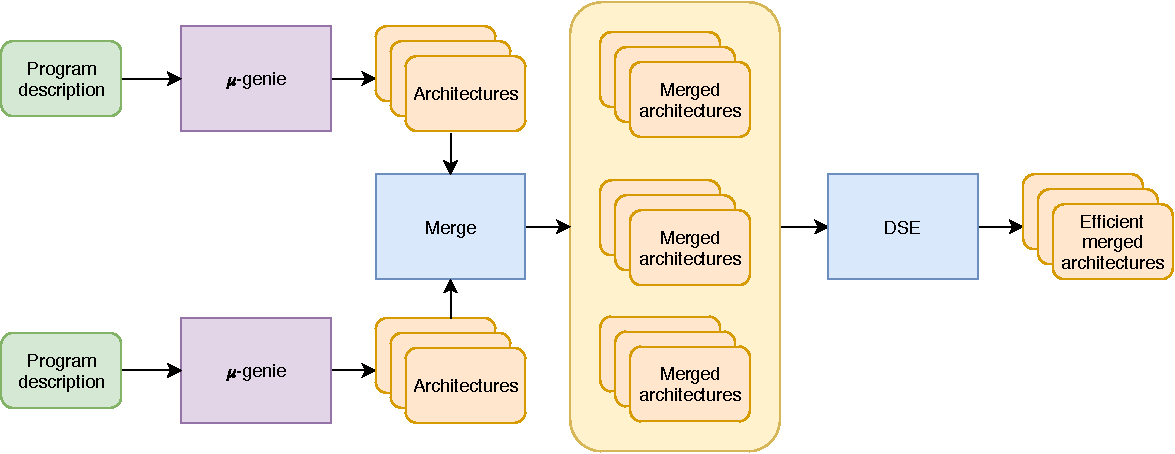
\includegraphics[width=\textwidth]{graphs/full_flow.pdf}
    \caption{A view of our full merging flow. We use \microgenie to generate sets of architectures from the program descriptions. After merging these sets, we use a DSE process to find the merged architectures that are efficient.}
    \label{fig:full_flow}
\end{figure}

For DSE, we first define the design space as the complete set of possible architectures for the input applications, i.e., the Cartesian product of the sets of architectures for each input application. Doing so gives us access to pairs of architectures with different parameters for all of our efficiency metrics (area, latency, and energy consumption), ensuring the completeness of our design space.

Next, we analyse each merged architecture using our efficiency metrics. Because each resulting architecture is multi-mode, it has separate latency and energy metrics for each individual mode, because both of these metrics depend on the execution. By construction (as designed in Section~\ref{method:method}), the latency and dynamic energy of each mode are the same as in the original architecture, whereas the static energy \textit{changes}, because it depends on the area of the merged architecture.

Finally, in our exploration, we find the Pareto set of the merged architectures. To do this, we assume a scenario in which all modes run equally often, i.e., for every execution of application 1 there is also an execution of application 2. Under this scenario, we can approximate the latency and energy of the merged architecture as the sum of the latency and energy of both modes. We note that with this method, different exploration strategies can be used by changing the way the metrics are estimated according to the scenario.

Using this DSE approach, in which we explore merges of \textit{all} the individual architectures implementing \textit{each} of the two given applications, and \textit{select only the efficient ones}, we generalise from a method of merging two architectures to a method for merging two applications.

\section{Implementation}
\label{method:implementation}
This section presents the pseudocode and implementation details of the methods formulated in this chapter, accompanied by a running example that demonstrates the architecture merging method in practice, step by step. The input architectures for this example are shown in Figure~\ref{fig:running_example}.

\begin{figure}[!htb]
  \begin{subfigure}{\textwidth}
    \centering
    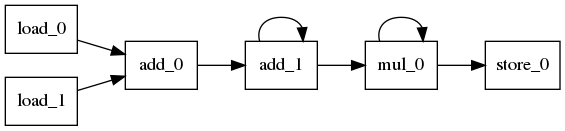
\includegraphics[scale=0.5]{graphs/running_example1.png}
    \caption{Architecture 1}
    \label{fig:running_example:a}
  \end{subfigure}\\
  \begin{subfigure}{\textwidth}
    \centering
    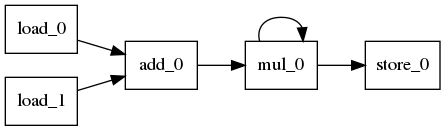
\includegraphics[scale=0.5]{graphs/running_example2.png}
    \caption{Architecture 2}
    \label{fig:running_example:b}
  \end{subfigure}
\caption{The input architectures of our running example. Architecture 1 has an extra \texttt{add\_1} node inserted compared to architecture 2.}
\label{fig:running_example}
\end{figure}

We calculate the \textit{mcs} on the input graphs with any self-edges removed. Since self-edges in the \microgenie output represent reads or writes from the component's own memory, these loops are irrelevant to the overall topology. However, the existence of loops in the graph would automatically mean that nodes containing them are non-isomorphic to nodes without them, and therefore cannot be matched as part of the \textit{mcs} algorithm. By removing such edges, we correctly maximise the coverage of the \textit{mcs}.

We find the \textit{mcs} by computing the maximum clique~\cite{konc2007improved}. on the compatibility graph between our two input graphs. We construct the edges of the compatibility graph by iterating over each pair of mappings in the compatibility graph, skipping any that map nodes of different types together. We add an edge between two mappings if they are \textit{compatible} (as defined in Section~\ref{bg:cg}). This construction is illustrated in Figure~\ref{fig:cgconstruction}. Each node in the maximum clique represents a pair of nodes, one from each input graph, which we map to each other to create the \textit{mcs}. Figure~\ref{fig:runningmcs} illustrates the \textit{mcs} for our running example.

\begin{figure}[!htb]
\begin{lstlisting}[title={Compatibility graph construction}, keywords={for, in, where, if, and}]
for vertex v1 in graph1:
    for vertex u1 in graph1, where v1 != u1:
        for vertex v2 in graph2, where v1.type == v2.type:
            for vertex u2 in graph2, where u1 != u2 and u1.type == u2.type:
                if edge_exists(v1, u1) == edge_exists(v2, u2):
                    add_edge(<v1,v2>, <u1,u2>)
\end{lstlisting}
    \caption{Pseudocode of the compatibility graph construction from two input graphs, where \texttt{v1} and \texttt{u1} are vertices in graph 1 and \texttt{v2} and \texttt{u2} are vertices in graph 2.}
    \label{fig:cgconstruction}
\end{figure}

\begin{figure}[!htb]
    \centering
    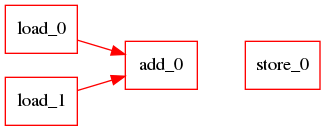
\includegraphics[scale=0.5]{graphs/running_example1+running_example2_mcs.png}
    \caption{The disconnected \textit{mcs} of the running example.}
    \label{fig:runningmcs}
\end{figure}

With the \textit{mcs} ready, we create the two leftover sets of nodes from each architecture by iterating over each node, adding any that are not part of the \textit{mcs} to the leftovers. We map the leftover nodes by type, and minimise the creation of new edges by selecting nodes with matching edges in the process. We do so by counting the amount of overlapping edges for each pair, and selecting the pairs with the most overlap. Edges are considered overlapping if the nodes connected to them map to each other, ignoring nodes that are not yet mapped. Figure~\ref{fig:mapping} shows the pseudocode for the matching algorithm, and Figure~\ref{fig:runningextended} illustrates the graph resulting from applying this to our running example, with the \textit{mcs} highlighted in red and the extended leftovers in blue.

\begin{figure}[!htb]
\begin{lstlisting}[title={Mapping leftovers}, keywords={for, in, where, if, while, and}]
while new pair possible:
    for vertex v in leftovers_in_graph1:
        for vertex u in leftovers_in_graph2, where v.type == u.type:
            overlap = 0

            for vertex a in adjacent_vertices(v):
                if equivalent_vertex_in_graph_2(a) in adjacent_vertices(u):
                    overlap += 1

            if overlap > max_overlap:
                best_pair = <v,u>
                max_overlap = overlap

    add_vertex_from_mapping(best_pair)
\end{lstlisting}
    \caption{Pseudocode of the mapping procedure for the leftovers.}
    \label{fig:mapping}
\end{figure}

\begin{figure}[!htb]
    \centering
    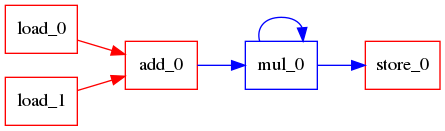
\includegraphics[scale=0.5]{graphs/running_example1+running_example2_extended.png}
    \caption{The \textit{mcs} of the running example extended with the mapped leftovers.}
    \label{fig:runningextended}
\end{figure}

Finally, we add any unmatched leftover nodes to the result graph along with all of their edges. The result is a complete supergraph, as illustrated in Figure~\ref{fig:runningfinal}. We see that both original input graphs are present in this final result graph.

\begin{figure}[!htb]
    \centering
    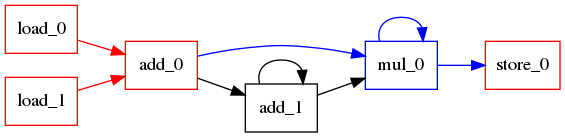
\includegraphics[scale=0.5]{graphs/running_example1+running_example2.png}
    \caption{The final result of the running example.}
    \label{fig:runningfinal}
\end{figure}

We perform our exploration over the Cartesian product of the sets of architectures created by \microgenie for each of the two input applications. For each pair in this set, we apply our merging method, resulting in a merged architecture, along with the mapping of each FU in the output architecture to one or two FUs in the input architectures. This information allows us to compute the metrics of the merged FU from its original FUs, enabling the exploration.

FUs differ in area depending on the area of the instruction memory, register files, and operation hardware. To be able to run both input programs, a merged FU must naturally have at least the area of the largest FU it was merged from. We compute the area of the merged FU as the maximum of the areas of the two original FUs. Similarly, the static energy per latency, which is based on the area, is the maximum of the original FUs. Finally, for the dynamic energy, which is only dependent on the FU's program, we use the original values.

To compute the total metrics for the merged architecture, we sum the individual metrics of all FUs in the architecture. In accordance with the scenario outlined previously (see Section~\ref{method:dse}), we sum the latency of both input architectures to obtain the latency we use for exploration, multiply it with the sum of the static energy per latency to obtain the overall static energy, and add to it the sum of the dynamic energy to obtain the total energy of the architecture.

We note that the area calculation for FUs outlined above is slightly simplified. As the area of the FU is the sum of the areas of the OP, RFs, and IM, each of which can vary depending on the bit sizes used and the FUs program, it would be more accurate to sum the individual maximum area of each sub-component. This is potentially relevant in certain edge cases where one sub-component is larger in one input FU and another sub-component is larger in the other. Additionally, we do not yet take into account the area increase created by increasing the amount of inputs to an FU, either due to increased crossbar hardware or due to the increased instruction memory size required for addressing. These discrepancies may minimally affect the result of the area calculation.
